\documentclass[prb,preprint]{revtex4-1} 

\usepackage{graphicx}
\usepackage{hyperref}
\usepackage{amsmath}
\usepackage{amsfonts} % needed for bold Greek, Fraktur, and blackboard bold
\usepackage{amssymb}
\usepackage[margin=1in]{geometry}
\usepackage{dcolumn}
\usepackage{multirow}

% TODO: remove these lines, which expand the margins (useful for comments)
\textwidth  .72\paperwidth
\hoffset -1in
\oddsidemargin .14\paperwidth
\evensidemargin .14\paperwidth
\marginparwidth .11\paperwidth


% Draft macros
\usepackage[normalem]{ulem} % for strikethrough
\usepackage[usenames,dvipsnames]{xcolor}
\newcommand{\TODO}[1]{\marginpar{\raggedright\scriptsize\textbf{TODO:} #1} (\textbf{TODO})}
\newcommand{\NOTEMARG}[1]{\marginpar{\raggedright\scriptsize\textbf{NOTE:} #1} (\textbf{NOTE})}
\newcommand{\NOTE}[1]{\marginpar{\footnotesize\textbf{NOTE}} (\textbf{NOTE: #1})}
\definecolor{purple}{rgb}{1,0,1}
\newcommand{\calvin}[2]{\textcolor{purple}{\sout{#1}#2}}

\newcommand{\eq}[1]{eq.~\eqref{eq:#1}}
\newcommand{\eqs}[2]{eqs.~\eqref{eq:#1} and \eqref{eq:#2}}
\renewcommand{\sec}[1]{section~\ref{sec:#1}}
\newcommand{\secs}[2]{sections~\ref{sec:#1} and \ref{sec:#2}}
\newcommand{\subsec}[1]{section~\ref{subsec:#1}}
\newcommand{\subsubsec}[1]{section~\ref{subsubsec:#1}}
\newcommand{\app}[1]{appendix~\ref{app:#1}}
\newcommand{\fig}[1]{figure~\ref{fig:#1}}
\newcommand{\figs}[2]{figures~\ref{fig:#1} and \ref{fig:#2}}
\newcommand{\tab}[1]{table~\ref{tab:#1}}
\newcommand{\nn}{\nonumber}

\newcommand{\FIGstudents}{
\begin{figure}[t]\center
\includegraphics[width=\columnwidth]{FIGstudents.pdf}
\caption{\label{fig:students} Students from the 2012 Compass Project summer program with model slinkies built out of washers and rubberbands.}
\end{figure}
}


\newcommand{\FIGpulsedrop}{
\begin{figure}[t]\center
\includegraphics[width=\columnwidth]{FIGpulsedrop.pdf}
\caption{\label{fig:pulsedrop} A few frames from a slow motion image of a wave pulse sent down a slinky next to a falling slinky.  Possible a graph of position vs time of the top of the falling slinky and the wave pulse.}
\end{figure}
}


\begin{document}

\title{A tale of two slinkies: learning about model building in a student driven classroom }
\author{Calvin Berggren}
\email{calvin1414@berkeley.edu}
\author{Punit  Gandhi}
\email{punit\_gandhi@berkeley.edu}
\author{Jesse Livezey}
\email{jesse.livezey@berkeley.edu}
\author{Ryan Olf}
\email{ryanolf@berkeley.edu}
\affiliation{Department of Physics, University of California at
Berkeley, Berkeley, California 94720, USA}
\date{\today}

\begin{abstract}

We describe a set of conceptual activities and hands-on experiments based around understanding the dynamics of a slinky that is hung vertically and released from rest.
The motion, or lack thereof, of the bottom of the slinky after the top is dropped challenges students' expectations and provides motivation and context for learning about scientific model building.
%This curriculum was developed for a week-long summer program for incoming freshmen as a part of the Compass Project~\cite{albana2013},
%The summer program is the first part of a three-course sequence aimed at helping incoming students in the physical sciences develop their identity as scientists.
This curriculum helps students learn about the model building process by giving them an opportunity to enlist their collective intellectual and creative resources to develop and explore two different physical models of the falling slinky system. By engaging with two different models, students not only have the opportunity to understand an intriguing counterintuitive phenomenon from multiple perspectives, but also learn deeper lessons about the nature of scientific understanding, the role of physical models, and the experience of doing science. 
The sequence of activities we present were developed for a week-long summer program for incoming freshmen as a part of the Compass Project,~\cite{albana2013} but could easily be implemented in a wide range of classrooms at the high school and introductory college levels.
\end{abstract}

\maketitle

\section{Introduction}
\NOTE{Rework this paragraph. Make sure to discuss about slinky being surprising enough to motivate the students and to ``level the playing field'' and
simple enough to accommodate widely varying backgrounds.}
This curriculum was developed for an intensive one-week summer program for
incoming freshmen as a part of the Compass Project.~\cite{albana2013,Roth2012,drdf2013a,drdf2013b}
The course was presented in a student-driven classroom
where the role of the instructors is to facilitate discovery and not lecture.
An important aspect of this type of classroom is that the students developed the models
themselves and took ownership over them. This is possible in a classroom with varying science
and math backgrounds because the topic was not a typical high school problem and required
many different skills to analyze.

The basis for the curriculum presented in this work is an experiment involving a
slinky that is hung vertically and released from rest. As the
slinky falls, the bottommost portion remains at rest and may seem to defy gravity\TODO{Should there be discussion of how we refined our question? Discuss the center of mass ideas we did?} until the remainder of the
slinky has fallen down to it.
The ``slinky drop''\NOTEMARG{Add multi-frame figure with labels.} experiment and other related phenomena have
been studied in detail,~\cite{calkin1993, newburgh1995, graham2001, aguirregabiria2007,unruh2011, cross2012}
and the recent flurry of interest in the slinky online \cite{..}
are a testament to the curiosity of the subject.
The lack of motion of the bottom of the slinky
served as an interesting, challenging, and counterintuitive phenomenon which our students sought to explain through
the construction of physical models. The phenomenon proved to be very well suited to
teaching the model building process in physics. In this work,
we seek to describe how we used the slinky drop to give the students first-hand
experience constructing two different physical models.

%%% The paragraph below is probably more detailed than we need to be about the structure of the program.
% The cirriculum is built around a central question that the students investigate.
%  This central question actually evolves throughout the course of the week as
% student gain understanding and develop a repetoir of scientific tools and
% methods.  The question may start out as "Does the slinky defy gravity?" and end
% up  "How does the bottom of the slinky know when to start falling?"

During the course of the program, we were able to approach the slinky using two different
and highly complemetary models.
One approach, detailed in \sec{forces}, approximated
the slinky by dividing it into discrete masses connected by simple springs and used
forces and Newton's Laws to calculate the motion of these masses.
We also made use of a complementary
model based on information, detailed in \sec{information}. This approach attempted
to describe the event when the slinky was let go as a piece of information which
needs to travel to other parts of the system before they are able to respond.
As expected, information proved to be a much more sophisticated concept for the
students to grasp but provided a clearer way of understanding why the bottom
is stationary. After presenting each
model individually in \secs{forces}{information}, we compare the models and
discuss model building in general in \sec{discussion}.
% Finally, our conclusions are presented in \sec{conclusion}.

\section{Modeling the slinky using forces}
\label{sec:forces}

In this model, we sought to use forces and Newton's Laws to calculate the
motion of the slinky. In order to make this brute-force approach more tractable, we
modeled the slinky as a series of discrete masses connected by simple springs, as
shown in \fig{discrete}. This
model was conceptually very straightforward and allowed the students to follow an
intuitive reductionist approach where they could divide the slinky into individual
constituents. Students were then able to apply familiar concepts in deciding how to model each part. Although the model turned out to
be formidable to solve for a nontrivial number of masses, it was still highly beneficial as it was restricted to the
use of elementary physical concepts, which built up into a larger, more interesting
phenomenon. Students were able to see how the different parts interacted and led
to the suprising behavior of the slinky.

% The strategy  was to find the forces (gravity and elastic) acting on 
% each mass as a function of position and then
% apply Newton's Laws to find the resulting motion.

%% no need for outline
% We then attempted to solve the equations
% of motion numerically to find the motion (\subsec{forcesnumeric}).

\subsection{Experimentally testing the simplified model}
\label{subsec:forcesexperiment}

\NOTE{Intro by discussing the need to see the extent to which this model
is applicable. Also reshuffle line below.}

We approached this model
by building a series of discrete masses as described above and taking measurements of
the motion.

\NOTE{Comparing the physical realization of the model to the slinky 
helps emphasize the distinction between the model and the actual phenomenon of interest.}

%Can the this simplified model based on physics that we understand actually explain a phenomenon
%in which the very physics in the model seems to be defied?

The students, with a little coaxing, decided that this could be done experimentally.  They built an 
apparatus that is closely described by the simplified model, so that they could compare its behavior to that of the 
actual slinky.  This was accomplished by tying metal nuts and washers (discrete masses) to 
rubberbands (springs), examples are shown in Fig. \ref{fig:students}.  

%\FIGstudents

The process of attempting to recreate the aspect of the slinky drop of interest using washers and rubberbands  
gave students some insight into the physical properties of the slinky that allowed for the bottom to  remain 
stationary when the top was released.  In particular, the students realized that the models must be very "stretchy"
in order to for this phenomenon to happen.  The students further realized how extremely stretchy the slinky is 
relative to other objects.

\begin{figure*}[t!]
  \centering

  \begin{tabular}{cccc}
    \multicolumn{2}{c}{
      \multirow{2}{*}{
        \raisebox{0\height}[0.6\height]{
          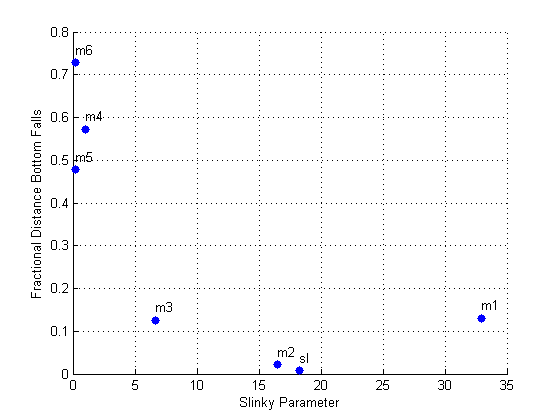
\includegraphics[width=0.5\textwidth]{figs/SlinkyParameter}
        }
      }
    } &
    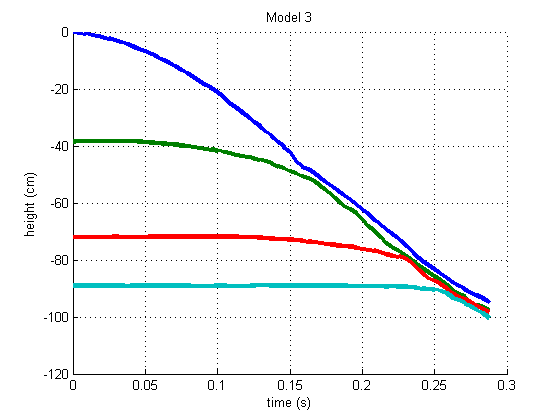
\includegraphics[width=0.25\textwidth]{figs/Slinky3} &
    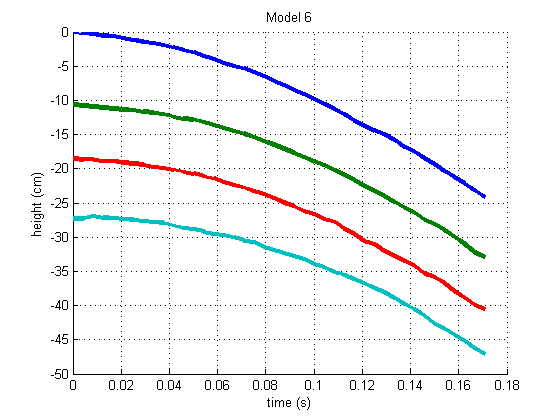
\includegraphics[width=0.25\textwidth]{figs/Slinky6} \\
    \multicolumn{2}{c}{} &
    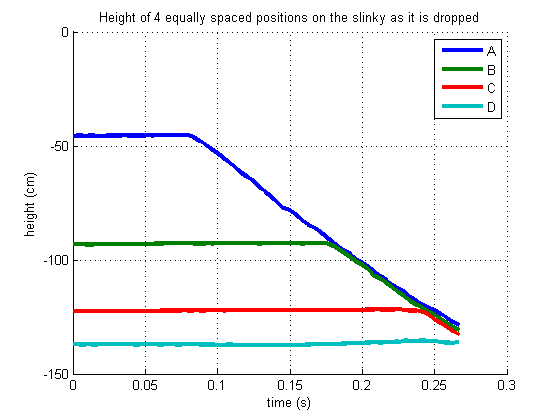
\includegraphics[width=0.25\textwidth]{figs/SlinkyTabs} &
    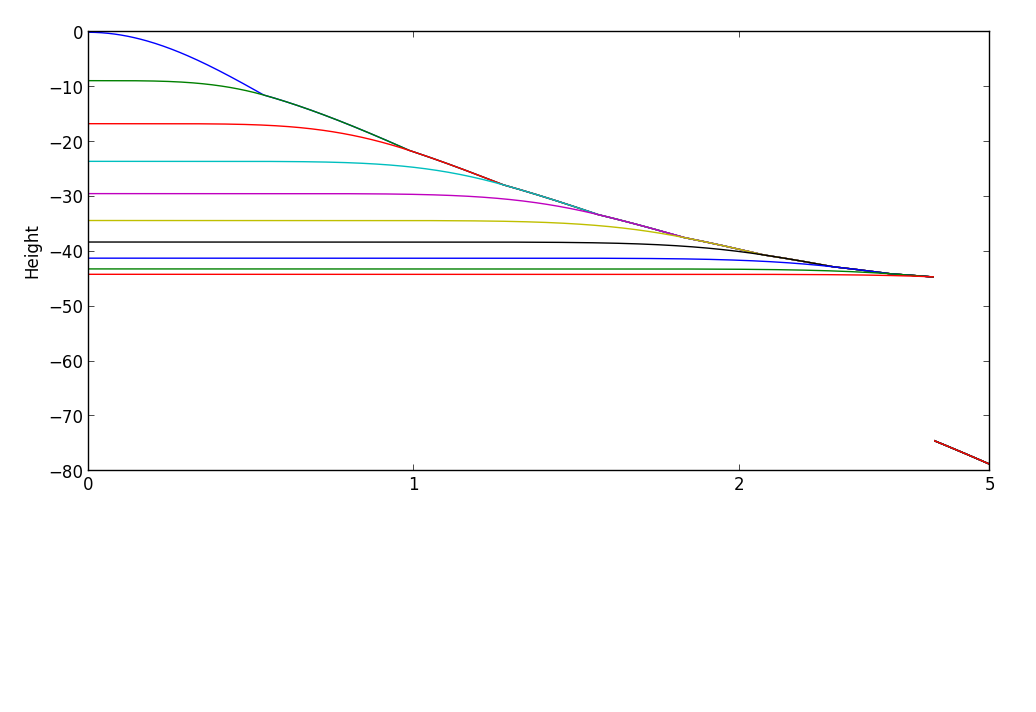
\includegraphics[width=0.25\textwidth]{figs/SlinkySim} \\

  \end{tabular}

  \caption{The left panel shows the correlation of the slinkiness parameter with
           how stationary the bottom mass is. Specifically, the extent to which the
           bottom mass is stationary is measured as the distance the bottom mass falls
           reletive to the stretched length of the system, during the time in which
           the top mass falls the full stretched length. The set of figures in the
           right panel shows the position as a function of time of four positions
           on the system. The top left is Model 3, the top right is 4 masses connected
           by strings, the bottom left is the slinky, and the bottom right is a
           simulation of Model ?.}
  \label{fig:discretemodel}
\end{figure*}

\TODO{Motivate this defninition.}This stretchiness can be characterized by how much the object stretches
under it's own weight as it is suspended.   We can define a slinky parameter as a measure of this:

\begin{equation}
\mathcal{S}=\frac{L_h-L_0}{L_0}
%\mathcal{S}=\frac{m g}{k_\text{eff} L_0 },
\end{equation}
where $L_h$ is the stretched length when suspended vertically and allowed to come to rest, and $L_0$ is the unstretched equilibrium length
when no forces act on it.  It can be shown using Newton's Laws that in the case of the discrete masses and springs model,
this stretching is actually proportional to the total mass $m$ and inversely proportional to the total effective spring constant $k_{\text{eff}}$ of the object.
This is also true in the case of a continous model of the slinky that can support the transmission of waves.  The following dimensionless quantity
can be constructed from the parameters of interest in the problem,
\begin{equation}
\mathcal{S'}=\frac{m g}{k_\text{eff} L_0 },
\end{equation}
 and is infact proportional to the  slinky parameter defined above.  Here, $m$ is the total mass of the object, $g$ is the gravitational acceleration felt as it is suspended, $k_\text{eff}$ is the effective spring constant of the entire object, and $L_0$ is the unstretched length.  It can be a useful activity to experimentally 
confirm this proportionality, particularly when the target audience hasn't been previously exposed to Newton's laws.

Now, in order to see that this parameter is a useful determining the "slinkiness", we must first choose a measure that allows us to compare how closely a model
with a given set of parameters behaves like a slinky in the drop experiment.  Since the phenomena of interest is the lack of motion of the bottom of the slinky, 
a good candidate could be the distance the bottom of the model falls in the time it takes for the model to collapse.  Figure \ref{} shows a plot of this distance, normalized by the stretched length unstretched length amount the object has stretched, for models over a range of different slinky parameters.  The slinky and simulations are also included in this graph.  One can see that the greater the slinky parameter, the less the bottom moves.  (or is there a threshold slinky parameter where  the bottom doesn't move beyond?).  We considered models with 4 masses, and have also shown the positions of the four masses as a function of time.  In order to facilitate comparisons between the models, the positioins have been normalized by the stretched length $L_h$, and the time is measured in units of $\sqrt{m/k_{\text{eff}}}$ of each of model.  

% \begin{table}[ht]
% \caption{Model Slinkies} % title of Table
% \centering % used for centering table
% \begin{tabular}{c c c c c c} % centered columns (4 columns)
% \hline\hline %inserts double horizontal lines
%  & m (g) & $k_\text{eff}$ (N/m) & $L_0$ (cm) & $L_h/L_0$ & $\mathcal{S}$ \\ [0.5ex] % inserts table 
%heading
% \hline % inserts single horizontal line
% model 1 & 405 & 0.7 	& 17   & 10	& 34		\\ % inserting body of the table
% model 2 & 205 & 0.7	& 17   & 9.5	& 17		\\
% model 3 & 200 & 2.1	& 14   & 6.5	& 7		\\
% model 4 & 30   & 2.1	& 14   & 2.0	& 1		\\
% model 5 & 200 & 60	& 16   & 2.1	& 0.2		\\
% model 6 & 200 & 75	& 16   & 1.7	& 0.17		\\
% slinky     & 190 & 1.7   & 5.7   & 24	& 19.6		\\ [1ex] % [1ex] adds vertical space
% \hline %inserts single line
% \end{tabular}
% \label{table:slinkies} % is used to refer this table in the text
% \end{table}
 


\subsection{Numerically testing the simplified model}
\label{subsec:forcesnumeric}

\NOTE{Add info somewhere about how it is possible to tune parameters with this model}

Having taken the step toward understanding the slinky using a model with
discrete masses separated by springs, we sought to make further progress by
solving this model numerically. The students spent some time constructing the
force equations for an $N=4$ system, which are
%%%
\begin{align} \label{eq:coupleddes}
m\ddot{x}_1 &= mg + k(x_2 - x_1)\,,
\nn\\
m\ddot{x}_2 &= mg + k(x_3 - x_2) - k(x_2 - x_1)
\,,\nn\\
m\ddot{x}_3 &= mg + k(x_4 - x_3) - k(x_3 - x_2)
\,,\nn\\
m\ddot{x}_4 &= mg                - k(x_4 - x_3)
\,,\end{align}
%%%
\NOTEMARG{\calvin{}{include \eq{coupleddes}?}}where $m$ is the mass of each discrete mass, $k$ is the spring constant of each
spring, $x_i$ refers to the absolute position of each mass, and the dots refer to
derivatives with respect to time.

Doing any serious exploration of these coupled differential equations
analytically was beyond the level of our audience; however, we briefly allowed
the students to consider how they would solve the system in order to demonstrate
the great difficulty of this strategy.

Students were gradually led toward an alternative numerical approach to solving
the problem that divided the evolution of the system into small time
steps. This was motivated by considering examples like the frames in a
movie\TODO{slow mo here and at the intro}. Discretizing time expanded on our previous decision to discretize the mass
in the slinky.

A major goal of this part of the curriculum was to show the benefits of building
numerical models. Not only does a numerical model
practically provide a way to make progress over an exact model which may be difficult
to work with, but these models also often provide a greater degree of transparency and
concreteness into how the system is evolving. We provided the class with the
ponderous analytical solutions to the 4-body system after the activity and asked
them how well they could see what was going on compared to the numerical
approach. We also asked how well they expected each approach to be able to
handle kinks or bends in the slinky to demonstrate the benefit numerical
approaches have in handling perturbations.\TODO{move below}

For the numerical approach, the students were asked to construct an algorithm
for how to proceed from one time step to the next. With the acceleration at each
step given by the force as in \eq{coupleddes}, the students settled on the
following simple algorithm (also known as the Euler method (Ref. \ref{..})),
%%%
\begin{align} \label{eq:algorithm}
v_i(t+\Delta t) &= v_i(t) + a_i(t)\Delta t
\,,\nn\\
x_i(t+\Delta t) &= x_i(t) + v_i(t)\Delta t
\,,\end{align}
with the time step given by $\Delta t$.

With the algorithm in hand, we had the students ``simulate'' the masses and
springs model as a group. Each mass was represented by a group of 
students, who completed the calculations for their mass to figure out where it would be
at the next time step.
% Students were divided into different roles, with some responsible 
% for calculation, others for communicating their position to other groups who 
% needed the information for their own calculations, and others for plotting the results on a graph 
% at the front of the room.
They would also plot their position on the board allowing the whole class to track
the progress of the simulation.
Groups needed information from other groups in order to complete their calculations,
and the communication of information between groups was intended 
to foreshadow the inherent time delay in the passing of information, explored later in
the week and described in \sec{information}.

One potential problem is that, for an $N$-body simulation and for the algorithm described in \eq{algorithm},
it will take $2N$ time steps for the bottom mass to move. This is not an explanation for
the lack of motion in the real slinky but is rather an artifact of the discretization of time:
the last mass will always wait $2N$ time steps regardless of the size of the step.
This provides an opportunity to discuss one limitation of this model.\TODO{more below}
% One way to
% accelerate the activity would be to use a more accurate symplectic algorithm, such as the
% symplectic Euler algorithm (Ref. \ref{...}). This algorithm would require only $N$ steps to move the bottom
% mass, partially alleviating the tedium for the last group.

The participatory simulation described here provides good practice in building
a model by iteration and highlights the ability of the numerical approach to incorporate changes to the model. After beginning the activity, questions quickly arise, such
as what to do when a mass passes through another mass. Nothing in \eq{coupleddes} prevents
the masses from passing. The students may wish to allow this to happen as an approximation
or they may wish to modify their procedure, perhaps by somehow merging any two masses which have overlaped
in the most recent time step. Follow up questions for discussion or investigation include
the dependence of the simulation on the size of the time step, the number of masses,
and other parameters.

It is also possible to perform this activity using a spreadsheet, which allows the steps to be
calculated much faster, albeit less collaboratively. We had the students implement the algorithm on a spreadsheet once they
felt comfortable with the details of the process. This allowed them to explore some of the follow
up questions more efficiently.

\section{Modeling the slinky using information}
\label{sec:information}
Coming from the numerical simulation of the masses and springs model, the students realize
two things. First, the numerical model has an artifact that causes the bottom mass to stay stationary.
This should be viewed as a systematic problem with the model, and not a prediction of the model.
\NOTEMARG{\calvin{}{I feel like this aspect of the simulation should be glossed over.}}
Second, when enough time passes so that the bottom mass does move, it initially moves very little compared 
to the distance the upper masses have moved. At this point it becomes clear that the discrete model
is not leading the class to a clear solution to the problem of the falling slinky.

\NOTE{\calvin{}{Alternative intro}}In addition to the force-based model, a model based on information avails itself to
the slinky drop. This model offers a great deal of insight into the phenomenon while
managing to avoid much of the tedious intermediate calculations of the force-based
approach. The information approach can be summed up in the following question:
how does the bottom of the slinky ``know'' that the top has been released? We sought
to address the fundamental limitation of how fast the information is able to propagate
down the slinky.

Initially, using ``information'' in the physics context may seem ill-defined and
abstract for the students. However, conceptual discussions had already alluded
unwittingly to what the bottom of the slinky ``knows'', and the wave properties
of the slinky had been discussed as well. 
We motivated a discussion of ``information travel'' in other contexts like earthquakes and tsunamis, 
lightning and thunder, sound, or slinky cows. Students were introduced to the idea that
this information that the top of the slinky had been dropped was being carried in a wave to the bottom
at some speed.\TODO{\calvin{}{emphasize the connection between the information and the waves}} Students investigated properties of waves, including the
effects of amplitude, frequency, tension, and material on wave propagation in slinkies.

This model for the slinky contrasted nicely with the previous model. The students were now thinking about
the slinky as a continuous object rather than a set of connected parts.

After the experimental activities, students were introduced to the method of dimensional analysis
to try and derive the speed of a wave on a slinky. They experimentally determined that the wave speed
seemed to be independent of frequency and amplitude, but that it did depend on the material from which
the slinky was made and the amount of tension placed on the slinkies. The quantities that the students
had left to work with were tension, $\tau$, and linear density, $\lambda$. Given these two quantities
the only quantity with units of velocity that can be created is:
\NOTEMARG{\calvin{}{I would say we scale back the discussion of the dimensional analysis
because for one, it did not work very well and second, we are not presenting
anything original here.}}
\begin{equation}
  \label{eq:wavespeed}
  v=\sqrt{\tfrac{\tau}{\lambda}}
\end{equation}
Characterizing the wave speed allowed us to place a concrete limitation on the amount
of time the information would take to travel from the top to the bottom. The question
now naturally presents itself of whether the top of a slinky in free fall would fall
faster or slower than a wave pulse. Based on the distribution 
of density and tension expected in a suspended slinky, the speed of the wave should decrease significantly as
it travels closer to the bottom of the slinky. On the other hand, the accumulated clump of slinky in free fall
continues to accelerate downward due to gravity and the tension in the slinky. It now seems plausible
that the clump might reach the bottom of the slinky before the wave can propagate to the bottom.

This can be verified experimentally. Two identical slinkies were suspended veritcally.
We permanently suspended one slinky and initiated a wave pulse starting at the top.
In this slinky, the medium does not collapse and only the pulse travels to the bottom. The other slinky was suspended and then dropped from the top. In this
slinky, a clump would accumulate as the slinky fell to the bottom. Using a slow-motion camera, the speed of the wave pulse
and the clump can be measured and compared.

\begin{figure*}[t!]
\begin{center}
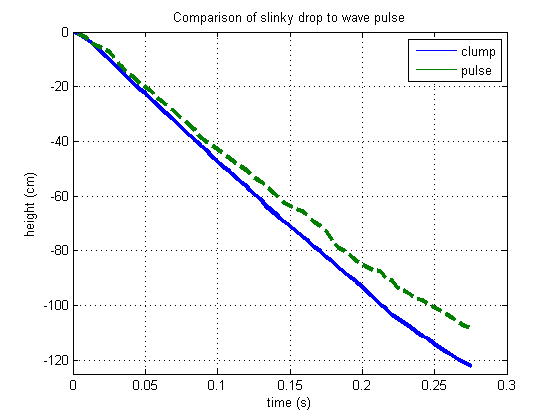
\includegraphics[scale=0.5]{figs/ClumpPulse}
\end{center}
\vspace{-4ex}
\caption{The position of a wave pulse on a suspended slinky compared to the position
of the top of an identical slinky when in free fall as a function of time.}
\label{fig:clumppulse}
\end{figure*}

The results of the measurements are shown in \fig{clumppulse}. These measurements
make clear that the falling top clump moves faster than a wave pulse on the same
slinky would. In a sense, the information-carrying wave pulse is being swallowed
by the slinky as it falls. We see this as the most natural way of understanding the
slinky drop. First, we understand that information travels at finite speed and so
the news of the release of the slinky will take time to propagate down the slinky.
Second, upon comparing the relevant constraints on the information travel for this
system, we find that the falling slinky exceeds this speed. This explains why the
bottom will still be stationary when the top arrives.

\NOTE{\calvin{}{I am in love with the torsional wave and almost can't resist mentioning it as a follow up question in this section.}}

\section{Discussion of Two Models}
\label{sec:discussion}

%% Old line from intro
% Despite the conceptual simplicity of the force-based model, the explanation
% required a large number of logical steps and a difficult calculation to arrive at
% the final conclusion. 

The fact that the slinky drop lends itself so naturally to two very different models
makes it an excellent backdrop for teaching model building. Having explored both
models, students are able to compare and contrast what kinds of insight are
offered by each one. Which model seems to apply more directly to the overarching
question of the ``levitation?'' Which model uses more basic concepts? Which model
better allows one to see the intermediate evolution of the slinky as it falls?
The models use different fundamental concepts and rules and approach
the problem in very different ways, yet obtain the same results.

Students often approach physics assuming that there is a single ``correct'' way
of looking at a problem. We sought to combat any expectation that we would
provide the ``right'' well-defined model and leave the students to solve it within
comfortable boundaries.
The students constructed a model on their own from basic underlying
principles, figuring out the best perspective to take, selecting which effects
to take into account, and determining which approximations to make.
We then took advantage of the slinky to force the students to attack the problem
from a different angle. Constructing a different model showed the students
how the set of decisions they made the first time around was not necessarily
\emph{the} unique way of approaching the problem. Multiple acceptable and potentially
useful approaches were possible for describing the same phenomenon.
% \TODO{\calvin{}{Lots of references are warranted in this paragraph.}}
\TODO{Lots of references are warranted in this paragraph.}

Each model makes different parts of the underlying physics
more transparent. The details of the interactions between the successive coils
of the slinky is manifest in the force-based model while the fundamental
limitation in the speed of information travel is less obscured in the model
using waves. Advantages of the force-based model included the students' ready
familiarity with the basic concepts of mechanics required and the straightforward
nature of the strategy of breaking the system into component parts. There were
fewer conceptual hurdles to overcome in this approach, and the mediating
reactions in the middle of the slinky were easy to see. 

Ultimately however, we feel that the information-based model provided the
most direct explanation for the levitation of the bottom of the slinky, albeit
using more sophisticated concepts. It focused
on the most relevant concepts for the question and abstracted away
nonessential parts. The great insight provided by the
model demonstrates the idea that the most useful models
capture only the effects that we are most interested in explaining.

Being able to readily attack the slinky drop from multiple angles, combined with
the fact that the slinky was simple enough to be approachable by the students
in a hands-on fashion, made it an ideal centerpiece of a curriculum intended to
introduce students to model building and allowed us to highlight many of the
essential features of model building in science.


\acknowledgments The authors would like to acknowledge helpful discussions with
D. R. Dounas-Frazer and J. Corbo along with the support of the Compass Project
community.

\NOTE{Fix person and tense}
\NOTE{Fix grammar and proofread!}
\NOTE{change ``model-building in science'' to ``physical sciences'' and other similar things}

\bibliography{slinky_bibliography}

\end{document}
